Dado los resultados de la sección anterior, se aplica QAOA al problema descrito en el artículo\cite{solving_shortest_path_with_qaoa}, con el fin de seguir analizando el comportamiento del algoritmo al aumentar el número de capas.

Este problema consiste, de nuevo, en obtener el camino más corto para un grafo, en este caso el desarrollado en la \textit{sección~\ref{sec:4-zhiqiang}}.

\subsection{Resultados con QAOA}

\begin{table}[Resultados QAOA {--} artículo de Shan et al.]{tab:5-zhiqiang_mod-orig_estadisticas}{Ejecución de QAOA del camino más corto en grafo del artículo\cite{solving_shortest_path_with_qaoa}}
  \centering
  \begin{tabular}{|c|r|r|}
    \hline
    \textbf{nº Capas} & \textbf{NA/TE} & \textbf{MM/TE} \\ \hline
    p = 1 &  0.1\% &  9.79\% \\ \hline
    p = 2 & 10.0\% & 20.20\% \\ \hline
    p = 3 & 38.1\% & 19.47\% \\ \hline
    p = 4 &  0.7\% & 27.33\% \\ \hline  % el 99.3\% de resultados ha sido 0101 (en lugar de 1010)
    p = 5 & 40.6\% & 24.29\% \\ \hline
    p = 6 & 30.7\% & 29.29\% \\ \hline
    p = 7 & 49.3\% & 24.60\% \\ \hline
    p = 8 & 71.4\% & 36.34\% \\ \hline
  \end{tabular}
\end{table}

A diferencia de las ejecuciones del grafo correspondiente a la \textit{tabla~\ref{tab:5-primer-paper-aer_estadisticas}}, aquí se ve un claro incremento de los aciertos (\textbf{NA/TE}) con el aumento del número de capas hasta que parece estabilizarse para el 40\%.

Se encuentra también el caso especial de $p = 4$, en el que los aciertos del algoritmo bajan hasta un \textit{0.7\%}.
\\
Además, para $p \ge 2$ se aprecian unos valores de \textbf{MM/TE} que se mantienen elevados.
Esto quiere decir que en situaciones como $p = 4$, aunque solo se encuentre el camino óptimo un $0.7\%$ de las ejecuciones, la media de apariciones en los histogramas es inusualmente elevada.

El resultado de la función gamma es el mostrado en la \textit{fig.~\ref{fig:5-zhiqiang_gamma-fun_p-20}}:

\begin{figure}[Resultados QAOA {--} artículo de Shan et al. {--} función gamma para $P = 20$]{fig:5-zhiqiang_gamma-fun_p-20}{Función gamma del grafo del camino más corto del artículo\cite{solving_shortest_path_with_qaoa}}
  \centering
  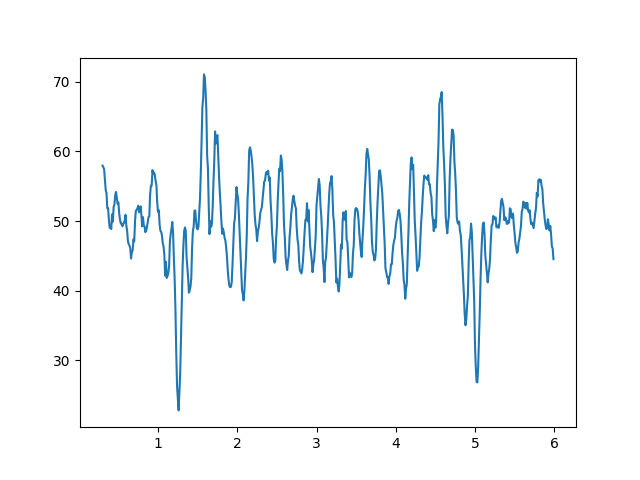
\includegraphics[scale=0.5]{zhiqiang-grafo/modificadores-paper/zhiqiang-p20-gammaFun.png}
\end{figure}

A diferencia de las funciones gamma de los problemas de max-cut (\textit{fig.~\ref{fig:5-tutorial-gamma_fun}}) y el camino más corto en grafo de 4 nodos (fig.~\ref{fig:5-primer_grafo/sin_restriccion_extra/primer_paper_p_27_gamma_fun}), en esta gráfica se ve mucho más ruido, pero también se aprecia cierta periodicidad a diferencia de la de la fig.~\ref{fig:5-primer_grafo/sin_restriccion_extra/primer_paper_p_27_gamma_fun}.

En la \textit{sección~\ref{sec:8-zhiqiang}} del apéndice se muestran otras pruebas realizadas sobre este grafo.

\subsection{Resultados de D-Wave}
\begin{table}[Resultados D-Wave {--} artículo de Shan et al.]{}{Resultados de la ejecución en D-Wave del grafo del camino más corto del artículo\cite{solving_shortest_path_with_qaoa}}
  \centering
  \begin{tabular}{|c|r|r|}
    \hline
    \textbf{Camino}        & \textbf{Energía} & \textbf{Muestras} \\ \hline
    1010 (\textbf{Óptimo}) &  7               & 776               \\ \hline
    0101                   & 12               & 247               \\ \hline
    0010                   & 46               &   1               \\ \hline
  \end{tabular}
\end{table}

Al igual que en anteriores ejecuciones utilizando \textit{quantum annealing}, se mantiene la coherencia en los resultados. El resultado obtenido un mayor número de veces es el camino óptimo y el siguiente camino más producido es el otro único camino válido (sin romper ninguna restricción).

\subsection{Resultados con librería de QAOA}

Las estadísticas ejecutadas con la función \textit{QAOAAnsatz} de Qiskit, al igual que en las secciones anteriores, muestran un comportamiento igual al obtenido en la implementación propia de QAOA (\textit{tabla~\ref{tab:5-zhiqiang_mod-orig_estadisticas}}).

\begin{table}[Resultados QAOAAnsatz {--} artículo de Shan et al.]{}{Resultados utilizando \textit{QAOAAnsatz} con el problema del artículo\cite{solving_shortest_path_with_qaoa}}
  \centering
  \begin{tabular}{|c|r|r|}
    \hline
    \textbf{nº Capas} & \textbf{NA/TE} & \textbf{MM/TE} \\ \hline
    p = 1 &  0.2\% &  9.86\% \\ \hline
    p = 2 &  1.2\% & 20.01\% \\ \hline
    p = 3 & 40.6\% & 19.62\% \\ \hline
    p = 4 &  0.5\% & 27.51\% \\ \hline
    p = 5 & 42.7\% & 24.88\% \\ \hline
  \end{tabular}
\end{table}


%%% Local Variables:
%%% mode: latex
%%% TeX-master: "../tfgtfmthesisuam"
%%% End:
